\item Se o caminhão acelera a uma razão constante de $\SI{6}{\meter/\second^{2}}$, partindo do repouso, determine a aceleração angular inicial da escada de \SI{20}{\kilogram}. A escada pode ser considerada como uma barra fina uniforme. O apoio em $B$ é liso.

\import{../answers}{answer-14}

\vspace{-1cm}
\begin{flushright}
	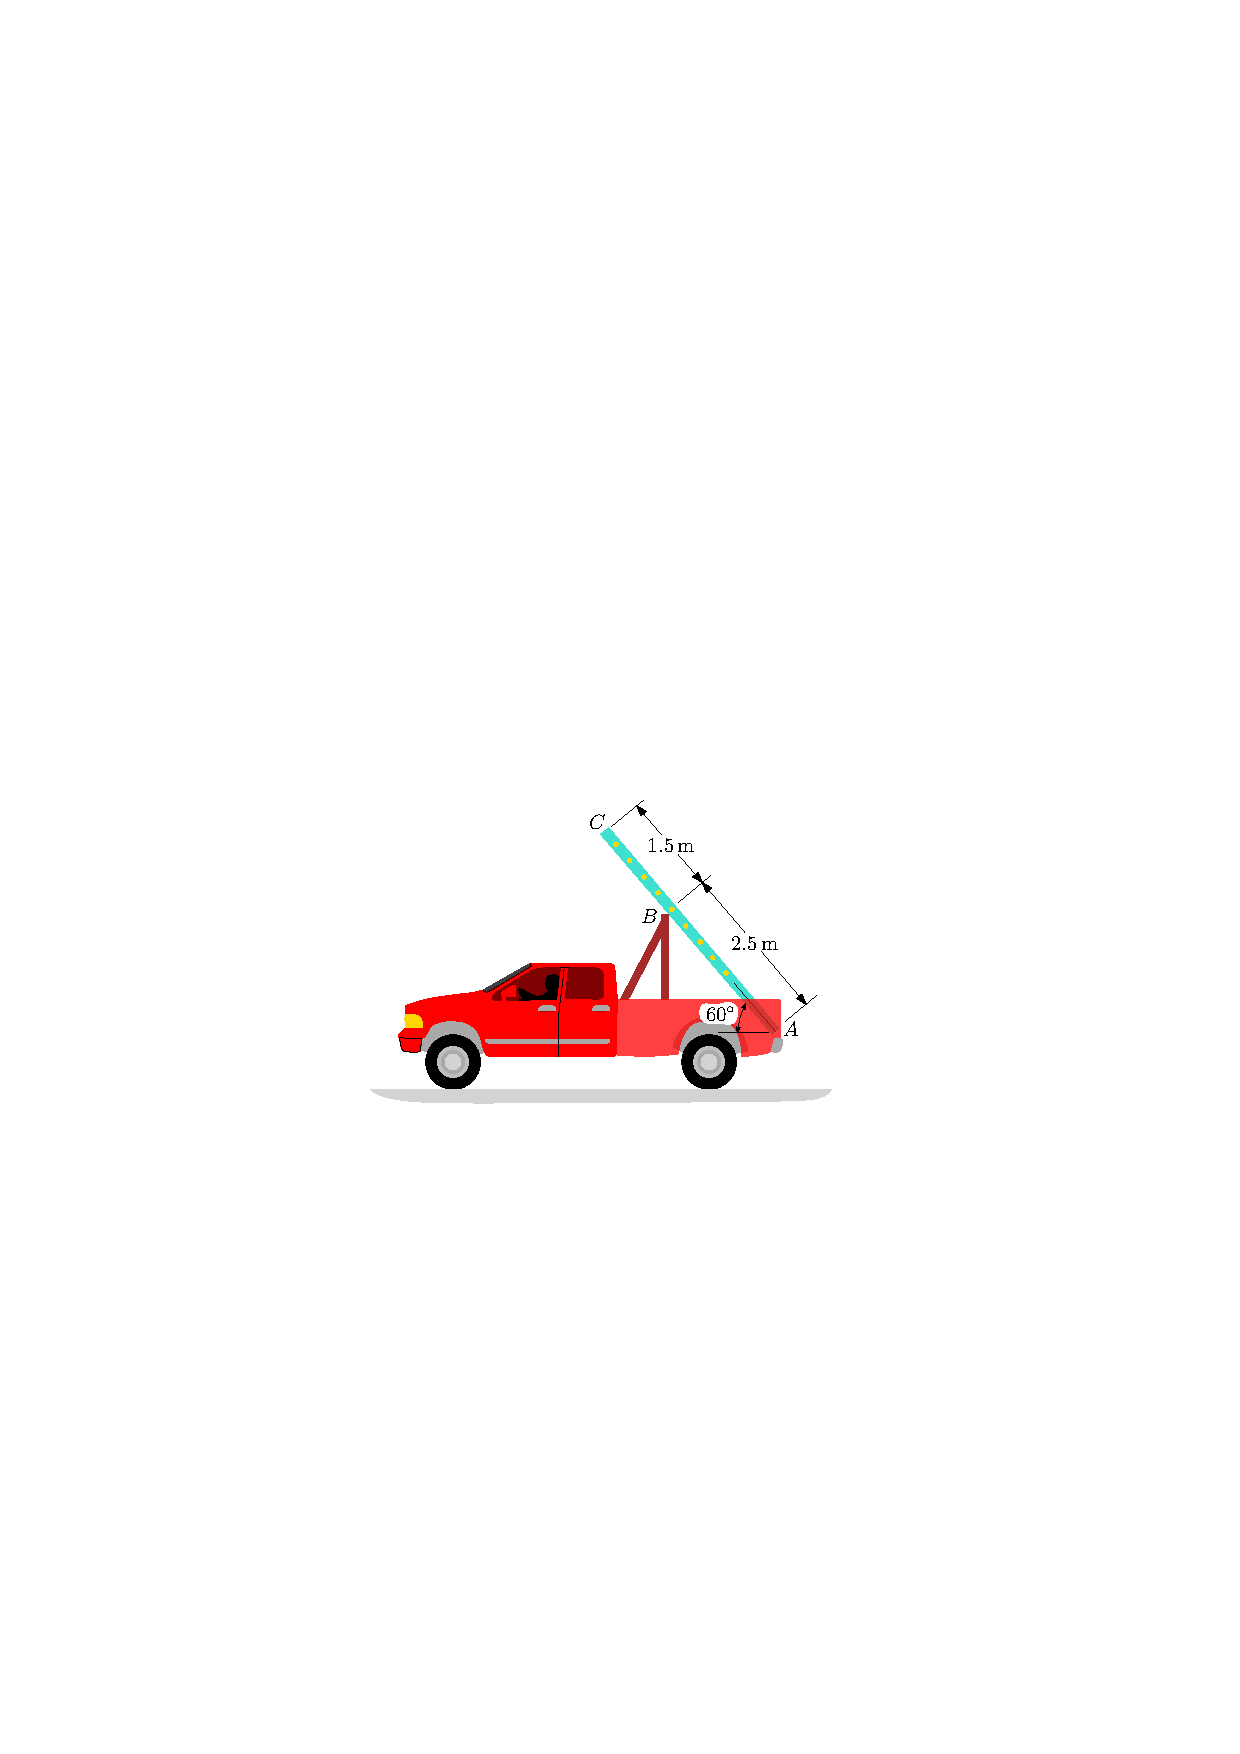
\includegraphics[scale=1.2]{../../images/draw_12}
\end{flushright}